\documentclass[11pt,a4paper,titlepage]{article}
\usepackage[utf8]{inputenc}
\usepackage[dutch]{babel}

\usepackage{color}
\usepackage{hyperref}
\usepackage{graphicx}

\title{Religie en zingeving oplossing examenvragen}
\author{Pieter-Jan Coenen}
\date{April 2017}


\begin{document}

\maketitle
\newpage
\tableofcontents
\newpage

\section{Kernbegrippen}
\subsection{Pale Blue Dot}
Pale Blue Dot is een foto van het heelal die genomen is door de ruimtesonde Voyager 1 na zijn missie op vraag van Carl Sagan. Op de foto is de aarde te zien op afstand van enkele miljarden kilometers. De aarde is op de foto nog maar een zeer klein blauw puntje in het gigantisch grootte heelal tussen alle andere sterren.\\
Sagen heeft ook zelf deze afbeelding becommentarieerd, het feit dat de aarde maar zo'n klein puntje is in het gigantische heelal deed bij hem bijvoorbeeld de vraag reizen waarom er wel een god geïnteresseerd zou zijn in dat super klein puntje (de aarde). Maar ook andere vragen zoals ``Wat moet de rol van de wetenschap zijn?'', ``Wat moet de rol van het geloof zijn?''  en ``Zou er toch meer zijn, zou er toch een God bestaan?''.

\subsection{Theïsme en deïsme}
Deïsme houdt in dat God de schepper van het universum en/of de aarde is, maar dat hij sinds de schepping op geen enkele wijze nog ingrijpt (God als 'horlogemaker').\\ Bij het theïsme daarentegen heeft God de aarde geschapen heeft en is deze na de schepping nog steeds betrokken.
\subsection{Theïstische evolutie (Collins)}
Collins is een verdediger van de theïstische evolutie, hij gelooft dat God de natuurwetten ingesteld heeft en dat de evolutie de manier is waarop hij zijn schepping realiseert.

\subsection{William Paley}
In zijn boek Natural Theology argumenteerde Paley dat er een God of toch een intelligent designer moet bestaan en dat de aanwijzigen hiervoor waren terug te vinden in de natuur. Hij vergelijkt de natuur met een uurwerk waarvan alle radartjes precies op elkaar afgestemd zijn. Bijvoorbeeld het oog van de mens zit zeer complex in elkaar.  Ook in de fysica speelt alles perfect op elkaar in. Uit het feit dat alles in de natuur zo perfect op elkaar is afgestemd besluit hij dat er wel een soort van intelligent designer moet bestaan.

\subsection{Natuurlijke theologie }
Natuurlijke theologie is het beargumenteren van het bestaan van een God m.b.v. aanwijzigingen uit de natuur, zoals bijvoorbeeld William Paley deed. In Paley's boek "Natural Theologie" vergelijkt hij de natuur met uurwerk, waarvan alle radartjes precies op elkaar afgestemd zijn. Bijvoorbeeld het oog van de mens zit zeer complex in elkaar.  Ook in de fysica speelt alles perfect op elkaar in. Omwille van deze complexe/vernuftige structuur van de natuur moet er wel een intelligent designer bestaan. \\ Darwin haalde later deze argumenten onderuit door de ontdekking van de natuurlijke selectie, de natuurlijke selectie bewijst dat de complexiteit gewoon gegroeid is.

\subsection{NOMA-principe}
NOMA = “non-overlapping magisteria” (Stephen J. Gould): de visie dat geloof en wetenschap twee onderscheiden domeinen zijn met eigen taak en autoriteit (wetenschap verklaart de werkelijkheid; geloof is bezig met levensvragen). Er kan daarom geen conflict zijn tussen beide.

\subsection{Wijsheid (volgens Stephen Jay Gould)}
Volgens Stephen Jay Gould is wijsheid aandacht geven aan zowel geloof als wetenschap. Voor Gould is er een scheiding tussen wetenschap en geloof. Maar kan je de echte wijsheid enkel bekomen door naar beide te kijken, we zijn pas wijs als we ze allebei kunnen integreren.

\subsection{Procrustesbed (Taede Smedes)}
Volgens Taede Smedes vormt de hedendaagse integratie van wetenschap en geloof (dus het feit dat ze met elkaar kunnen verzoend worden) vrijwel altijd een 
soort procrustesbed vormt, waarbij of de theologie of natuurwetenschap op maat wordt gesneden om compatibiliteit met de andere helft te garanderen.

\subsection{Pillenmaatschappij}
We willen gelukkig zijn, we willen zeer gelukkig zijn, eigenlijk veel te gelukkig zijn. Gelukkig zijn lijkt een levensdoel, lijkt het ultieme om te bereiken in ons leven. Wanneer we ons ongelukkig voelen gaan we daarom naar de psychiater, waar we vragen voor een pil, zodat we terug door het leven kunnen denderen. Doordat we zo gelukkig willen zijn, worden er ongeloofelijk veel pillen genomen. Het lijkt alsof onze maatschappij niet kan bestaan zonder deze pillen. We hebben een pilletje voor alles.

\subsection{Hedonistische adaptatie}
Hedonistische adaptatie is het fenomeen waarbij een verandering in onze omgeving (nieuw lief, nieuwe auto, loonsverhoging) slechts een korte tijd zorgt voor een hoger geluksniveau. Dit komt omdat we zeer snel wennen aan het nieuwe en terugvallen op ons oude geluksniveau

\subsection{Individualisering}
Individualisering betekent dat we meer zelf kunnen en moeten kiezen. We moeten zelf de managers van ons leven worden. Individualisering houdt vrijmaking in. Er liggen voor elk individu vele mogelijkheden open. We kunnen zelf kiezen welke we willen benutten. Er zijn dus meer mogelijkheden om te kiezen voor andere invullingen van onze identiteit, gebaseerd op alternatieve verhalen (= separatie). 

\subsection{Detraditionalisering}
Detraditionalisering betekent dat traditionele opvattingen, gedragingen en omgangsvormen gerelativeerd worden. Ze verliezen hun dwingend karkater, maar verdwijnen niet. Ze veranderen van sociaal dwingende opties in mogelijke mogelijkheden.

\subsection{Keuzebiografie}
Keuzebiografie heeft te maken met individualisering. Het dagelijkse leven wordt een aaneenschakeling van keuzes. Steeds minder ligt vast, door afkomst, door sociaal milieu, door de maatschappij. Je moet zelf veel meer nadenken over dingen zoals "wat wil je worden", "waar ga je wonen", "samen wonen of niet", ...
Al die vragen zijn mogelijkheden, opties waarover beslist moet worden. Vroeger daarentegen lag ons leven veel meer vast, het was veel felller uitgestippeld.
Geïndividualiseerde individuen worden niet meer beperkt door wat mensen in de buurt en religieuze leiders goed of fout vinden. Je kan zelf veel meer kiezen. Het kunnen kiezen betekend ook het moeten kiezen, je moet kiezen wat je gaat studeren, hoeveel kinderen je wil. Het leven is een aaneenschakeling van keuzes.

\subsection{Identificatie}
We spiegelen ons aan de anderen, nemen het dominante verhaal over. De maatschappij zegt ons wie we zijn, moeten zijn, niet mogen zijn. Overnemen van verwachtingen en opdrachten voor onze toekomst vanwege onze familie, onze sociale groep, onze cultuur, enz.

\subsection{Separatie}
Separatie is één van de twee processen die onze identiteit vorm geven. Het is de mogelijkheid te kiezen voor andere invullingen, gebaseerd op alternatieve verhalen. Het is de spiegel, die ons voorgehouden wordt, afwijzen. Impliceert relatieve keuzevrijheid en verantwoordelijkheid.

\subsection{Rank \& Yank}
Alle werknemers jaarlijks beoordelen op hun productiviteit, rangeer ze vervolgens en ontsla de 20\% slechtste werknemers, nadat je ze hebt vernederd. Dit zal de competitie en de productiviteit onder de werknemers doen stijgen. Dit zal zorgen voor een meer rendabel bedrijf. Een denkwijze uit het neoliberalisme, door de concurrentie op te drijven zal de rendabiliteit toenemen.

\subsection{Het individueel schuldmodel}
Dit is de dominante visie op mislukken in de hedendaagse samenleving. Slagen is slechts een kwestie van je best doen. Je kan het maken, dus je moet het ook maken. Wie faalt, heeft gewoon niet hard genoeg zijn best gedaan en heeft het dus enkel zichzelf te danken.

\subsection{Sociaaldarwinisme}

Het is ontstaan nadat Darwin de evolutie theorie had gepubliceerd. Het is de overtuiging dat deze evolutie theorie duidelijk maakt dat we competitie en concurrentie in de maatschappij moeten bevorderen. M.a.w. dat het goed is dat er een strijd is in het bestaan, omdat we daar dan met z'n alle beter van worden. Liefdadigheid, het zorgen voor zwakken is geen goed idee, want dan zorg je ervoor dat die langer blijven overleven en zich kunnen voortplanten naar volgende generaties en dat gaat uiteindelijk ten kosten van de soort, hier is dat dan de mensheid. \\ Volgens Paul Verheagen is het neoliberalisme een soort van sociaaldarwinisme.

\subsection{Gordon Gekko}
Gordon Gekko is een komisch personage uit de film "Wolf of Walstreet" dat in de les werd gebruikt als een voorbeeld van de neoliberale opvattingen. Om aan te tonen dat hebzucht en egoisme de fundamenten zijn van het evolutionaire denken, dat de evolutie theorie beargumenteerd dat wij met z'n alle concurrenten van elkaar moeten zijn.

\subsection{De zuilen van de moraliteit (volgens Frans de Waal)}
\begin{enumerate}
\item Wederkerigheid en rechtvaardigheid (fairness)
\item Empathie en compassie
\end{enumerate}

\subsection{De Baal Sjem Tov}
Vernam in een droom dat hij een gebod overtreden had en daarom het eeuwig leven ontzegd was. Was daar zeer blij mee want nu kon hij het goede doen omwille van het goede en niet omwille van enige beloning. Dit illustreert dat in het jodendom het doen het belangrijkste is. 

\subsection{Het dubbelgebod van de liefde}
Het kadert in het verhaal van de barmhartige samaritaan. Een schriftgeleerde gaat naar Jezus toe en vraagt hem wat hij moet doen om het eeuwige leven te krijgen. En dan antwoord Jezus met een betere vraag "Wat zegt de Thora daarover?". De geleerde antwoordt  dan met het dubbelgebod van de liefde, "het liefhebben van de heer god, met heel je hart, heel je ziel, heel je verstand en je naasten als jezelf".\\
Het dubbelgebod van de liefde vat eigenlijk de volledige Thora samen.

\subsection{Verantwoordelijkheid in de eerste persoon}
Het zorgen voor jezelf. Als eindig en kwetsbaar wezen heb je de opdracht jezelf in het bestaan te handhaven. Je moet bekommerd zijn om mezelf. Het leven is een opdracht. Je moet iets van je leven maken, moet de zorg voor jezelf opnemen en moet werk maken van een zinvol en gelukkig leven. 

\subsection{Verantwoordelijkheid in de tweede persoon}
Verantwoordelijkheid in de tweede persoon = verantwoordelijkheid voor de noodlijdende ander (“barmhartigheid”): De noodlijdende ander onderbreekt mijn zelfzorg. Als kwetsbaar en lichamelijk wezen word ik door zijn kwetsbaar en gekwetst lichaam geraakt. Ik verlies mijn vrijheid van initiatief, maar behoud wel mijn vrijheid van antwoord. Het gaat echter niet om twee gelijkwaardige alternatieven. De ander stelt mij voor hem verantwoordelijk, ik sta bij hem in de schuld. Als ik mijn verantwoordelijkheid niet opneem, dan sticht ik het ethisch kwade en heb ik morele schuld.

\subsection{Barmhartigheid}
Barmhartigheid is de ander in zijn lijden en sterven niet alleen laten. Je doet iets alsof het volledig gratuit is, je doet het voor iemand zonder dat je er iets voor terug zou krijgen. Je moet iedereen behandelen alsof ze dood zullen zijn tegen middernacht. Het mag ook niet iets zijn dat je puur uit medelijden doet. Het moet iets materieel, iets natuurlijk worden. Doordat de barmhartige samaritaan aan zelfzorg in de eerste persoon heeft gedaan, een vermogen heeft opgebouwd. Kan hij nu zorgen voor een ander. Barmhartigheid is hetzelfde als verantwoordelijkheid in de tweede persoon.

\subsection{Tragiek van de goedheid}
Wie helemaal ingaat op de roep van de ene noodlijdende ander langs de kant van de weg zal onvermijdelijk onrecht en zelfs geweld doen aan andere anderen die ook recht hebben op aandacht en zorg. Als je goed doet voor ene noodlijdende ander, dan is er een grote kans dat je iemand anders in de steek laat, niet kan helpen. Daarom moet rechtvaardigheid de barmhartigheid begrenzen.

\subsection{Verantwoordelijkheid in de derde persoon}
Door helemaal in te gaan op de nood van één unieke ander kunnen we onrecht doen aan “derden”, d.w.z. andere anderen , zij die in ruimte en/of tijd van ons verwijderd zijn. We moeten ook instaan voor de gevolgen van de acties, ookal gebeuren die veel later, ookal waren die niet te voorzien. De barmhartigheid moet met andere woorden begrensd worden door de rechtvaardigheid. 

\subsection{Midrasj}
Een midrasj is een interpreterend verhaal waarbij men elementen gaat toevoegen om het begrijpelijker, aannemelijker te maken. Men gaat dus eigenlijk de stukken waardat de tekst je in het ongewissen laat verder gaan invullen. Bijvoorbeeld Sarah die op het laatste moment haar status van getrouwde vrouw gaat bekend maken.


\section{Synthesevragen}

\subsection{Bespreek de drie klassieke modellen om de verhouding tussen geloof/religie en wetenschap te denken. }
\begin{enumerate}
\item Het conflictmodel stelt dat geloof en wetenschap concurrerende
alternatieven zijn. Je kan niet beide tegelijk aanhouden en moet dus
kiezen tussen beide. Dit is de positie van militante atheïsten zoals
Richard Dawkins, maar ook van aanhangers van het creationisme. 
\item Het kloofmodel probeert dit conflict op de lossen door te zeggen dat
geloof en wetenschap totaal verschillende benaderingen van de
werkelijkheid zijn die zo grondig verschillen dat ze niet met elkaar in
conflict kunnen komen. Zo verdedigt Stephen Jay Gould het NOMA-principe:
wetenschap beschrijft de werkelijkheid (hoe-vragen) en religie
houdt zich bezig met zinvragen (waarom-vragen). Probleem is dat
religie hier wel de zwaarste prijs betaalt (wetenschap bepaalt wat
religie nog kan zeggen) en het is nog maar de vraag of religie in
isolement kan blijven van de wetenschap. 
\item Het harmoniemodel probeert het conflict tussen geloof en wetenschap op te lossen door beide te integreren en ze in elkaar of in een overkoepelende eenheidstheorie te laten opgaan. Een verdediger hiervan is bijvoorbeeld Francis Collins die verdedigt dat God de natuurwetten ingesteld heeft en dat de evolutie de manier is waarop God zijn schepping realiseert. Volgens Taede Smedes leidt het harmoniemodel echter vaak tot nieuwe conflicten omdat de één op maat van de ander gesneden wordt om ze samen te laten passen. 
\end{enumerate}

\subsection{Hoe brengt Francis Collins geloof en wetenschap samen? Welke kritiek kan je op Collins geven met behulp van Frans de Waals TED-lezing? Op welke manier bevestigt de mogelijkheid van deze kritiek de visie van Taede Smedes op het probleem met integratie van geloof en wetenschap? }
Francis Collins is een voorstander van het harmoniemodel, hij probeert het conflict tussen geloof en wetenschap dus op te lossen door beide in elkaar te integreren m.b.v. een overkoepelde eenheidstheorie. Hij zegt dat God de natuurwetten ingesteld heeft en dat de evolutie de manier is waarop God zijn schepping realiseert, hij is dus een voorstander van de theïstische evolutie. Het beoefenen van wetenschap is dus in zijn ogen een manier om meer inzicht te krijgen in de schepping van God, een inkijk in de geest van God. Hij beschouwd het beoefenen van wetenschap zelfs als een soort van Gods aanbidding. Door aan wetenschap te doen kom je volgens zijn theorie immers meer te weten over de schepping van God, want voor de theïstische evolutionisten heeft God de evolutie en de wetten van de natuur geschapen. Je kan de diepere waarheid bekomen door geloof en wetenschap te combineren. Collins gebruikt ook het bestaan van moraal als bewijs van theïstische evolutie. Hij zegt dat er in ons een bepaalde moraal ingebakken is en dat  God ervoor heeft gezorgd dat we ook goed zijn voor elkaar. Hij is ervan overtuigd dat die moraal er al van het begin was. \\
Frans de Waal komt vanuit de wetenschap tot de tegengestelde conclusie. Hij bewijst juist dat de moraal van onderuit is gegroeid. Hij vergelijkt het met een Russisch poppetje met drie lagen. De binnenste laag is de oudste, de andere lagen zijn er dan later rond gekomen. Binnenste laag is de emotionele aanstekelijkheid. Deze is wijdverspreid in het dierenrijk, bv. muizen die pijn voelen als ze een andere muis pijn zien lijden. Tweede laag is er daarna bijgekomen, het geven van troost. Iemand die niet betrokken is in een gevecht gaat proberen iemand die betrokken is in het gevecht zijn gemoedstoestand te verbeteren. Derde laag, deze is het minst wijd verspreidt, de empatische perspectiefname. Dit is het instaat zijn om in te schatten wat een ander nodig heeft. Bijvoorbeeld een duiker die in de problemen is en wordt gered door een dolfijn. De drie lagen van empathie vormen voor Frans de Waal de bron van altruïsme. \\
Dit bevestigd dus ook de kritiek van Taede Smedes. Door beide met elkaar te proberen verzoenen wordt het ene op maat van het andere gesneden om compatibliteit te garanderen en kom je tot een nieuw conflict waarin het ene wordt beperkt door het andere.

\subsection{Bespreek de visie van Stephen Jay Gould op de verhouding tussen religie en wetenschap.
Wat wil Goud met zijn voorstel bereiken? Slaagt hij in zijn opzet (waarom wel/niet)?}
Stephen Jay Gould doet een poging om geloof en wetenschap te verzoenen, dit doet hij met het kloofmodel, wat wil zeggen dat volgens hem geloof en wetenschap totaal verschillende benaderingen van de werkelijkheid zijn die zo grondig verschillen dat ze niet met elkaar in conflict kunnen komen. Hij is de grondlegger van het NOMA-principe (“non-overlapping magisteria”). Het is de visie dat geloof en wetenschap twee verschillende domeinen zijn met eigen taak en autoriteit, wetenschap beschrijft de werkelijkheid (hoe-vragen, de feiten, de theorie) en religie houdt zich bezig met zinvragen (waarom-vragen). Omwille van die redenen suggereert Gould dat er geen conflict kan zijn tussen beide. \\ 
In het opzicht van religie slaagt hij niet in zijn opzet, omdat het probleem van deze houding is dat religie hier de zwaarste prijs betaalt (wetenschap bepaalt wat religie nog kan zeggen) en het is de vraag of religie in isolement kan blijven van de wetenschap. Het NOMA-principe beperkt de religie, want die moet zich aanpassen aan de wetenschap. Hij is er dus niet in geslaagd om beide te verzoenen, sterker nog hij lijkt zelfs een nieuw conflict te creeëren. \\
Zoals Taede Smedes stelt, vormt de integratie van wetenschap en geloof een procrustesbed, waarbij de theologie of de wetenschap steeds op maat wordt gesneden met het andere om compatibliteit te garanderen.

\subsection{Bespreek tekst van de standaard}
De resultaten van dit onderzoek komen duidelijk perfect overeen met de visie van Dirk De Wachter en Sonja Lyubomirsky op geluk. \\  \\
Het al dan niet hebben van een smartphone maakt dus duidelijk niet gelukkig. Dit heeft volgens Sonja Lyubomirsky te maken met hedonistische adaptatie. Wanneer je iets leuk koopt, iets geweldig meemaakt, dan zal dat je misschien enkele weken gelukkiger zal maken, maar daarna zal je steeds terug vallen naar een standaard niveau van geluk. Het al dan niet hebben van een smartphone, een spelconsole zal je dus niet op de lange termijn gelukkiger maken. \\
Ook Dirk de Wachter is ervan overtuigd dat we niet moeten streven naar geld, naar een dure auto, een groot huis, want het maakt ons eigenlijk toch niet gelukkiger, dat doet ons toch niet beter voelen. \\ \\
Het artikel zegt dat vrienden, een leuke meester of juffrouw ons daarentegen wel gelukkiger maken. Het hebben van een goed leven met veel vrienden, waarin we niet worden gepest en een mama en papa hebben waarbij we terecht kunnen zou er dus voor zorgen dat kinderen wel gelukkig zijn.\\
Dit sluit ook aan bij de visie van Sonja en Dirk. Sonja zegt dat je een goed leven moet leiden en dat geluk dan wel zal volgen. En deze studie maakt dus duidelijk dat dit inderdaad het geval is. Ook De Wachter bevestigd dit, hij zegt dat het ultieme doel van het leven niet is dat je een gelukkig leven moet leiden, maar dat je een goed leven moet leiden. \\ \\
Lyubomirsky is er ook van overtuigd dat geluk vooral genetisch bepaald is en dat iemand die de neiging heeft om altijd negatieve dingen te zien, het ook veel moeilijker zal hebben om gelukkig te zijn. Volgens haar kunnen we dus weinig veranderen aan ons geluksniveau, want de persoonlijkheid van iemand kan je niet zomaar veranderen. Mensen die van nature niet graag naar school gaan (niet omdat ze gepest worden of geen vrienden hebben), zullen dus altijd minder gelukkig zijn op school. Hun standaard geluksniveau waarnaar ze terug vallen is dus lager en daardoor zijn ze minder gelukkig op school. \\ \\
Volgens Dirk worden mensen ook ongelukkig omdat ze niet meekunnen met onze speedboot maatschappij, omdat ze niet de beste jobs hebben of de duurste wagen. Wanneer je dus een goede leerkracht hebt, die alle leerlingen gelijk behandeld en ervoor zorgt dat de kinderen met een lagere socio-economische afkomst extra worden ondersteund. Dan wordt het verschil tussen de kinderen kleiner en zullen ze dus bijgevolg gelukkiger zijn.



\subsection{Vergelijk de visie van Dirk De Wachter en Sonja Lyubomirsky op geluk. Waarover zijn ze het eens? Waarin verschillen ze van mening? Verwoord ook hoe jij aankijkt tegen hun beider visies. Beargumenteer je standpunt. }
Sonja Lyubomirsky spreekt over de twaalf geluksactiviteiten, deze gaan vooral over hoe je een goed leven moet leiden. Sonja is ervan overtuigd dat je een goed leven moet leiden en dat geluk dan wel zal volgen.\\ 
Dit komt overeen met de visie van De Wachter, hij zegt dat het ultieme doel van het leven niet is dat je een gelukkig leven moet leiden, maar dat je een goed leven moet leiden. Beide zijn er dus van overtuigd dat het leiden van een goed leven zeer belangrijk is. \\ \\
Sonja spreekt ook over hedonistische adaptatie, dit wil zeggen dat mensen heel snel gaan terug zakken naar een standaard niveau van geluk. Een bepaalde gebeurtenis kan er bijvoorbeeld voor zorgen dat we ons even gelukkiger voelen, maar daarna gaan we steeds terugvallen naar een standaard niveau van geluk. Omstandigheden hebben volgens haar dus maar een heel korte invloed op geluk.\\ 
Ook dit komt overeen met de visie van De Wachter, hij zegt dat we niet moeten streven naar geld, naar een dure auto, een groot huis, want het maakt ons eigenlijk toch niet gelukkiger, dat doet ons toch niet beter voelen. \\ \\
Lyubomirsky is er ook van overtuigd dat geluk vooral genetisch bepaald is en dat iemand die de neiging heeft om altijd negatieve dingen te zien, het ook veel moeilijker zal hebben om gelukkig te zijn. Volgens haar kunnen we dus weinig veranderen aan ons geluksniveau, want de persoonlijkheid van iemand kan je niet zomaar veranderen.\\ 
Dirk De Wachter daarentegen is ervan overtuigd dat ons geluk wel wordt bepaald door de omgeving. In onze "speedboot-maatschappij"  gaat er veel aandacht naar prestaties, geld, kleding enz. Dit zorgt ervoor dat veel mensen uit de boot vallen, zich afwegen t.o.v. andere die dit wel allemaal hebben en zich daardoor ongelukkig voelen.

\subsection{Wat kenmerkt onze samenleving? Hoe beïnvloedt onze samenleving ons geluk?}
Er zijn heel wat dingen die onze hedendaagse samenleving kenmerken. Dirk de Wachter beschrijft onze maatschappij als een maatschappij waarin alles perfect lijkt te gaan. Waarin iedereen super gelukkig wilt zijn en gelukkig zijn bijna het ultieme doel van het leven lijkt. \\ We willen de duurste auto's, het mooiste huis, de perfecte kinderen, de beste job. Het lijkt zelfs alsof geluk te koop is. Je kan heel veel kopen om je beter te doen voelen, je kan naar de welness gaan, je kan reizen. Het geluk lijkt wel bepaald door geld en we leven dus in een maatschappij waarin we het idee hebben dat alles te koop is. Als we maar succes hebben en veel geld verdienen, dan kunnen we een gelukkig leven leiden. We streven allemaal naar dat ultieme succes, het perfecte leven. Iedereen moet presteren en moet het goed doen. \\
Wanneer we deze ultieme droom niet kunnen bereiken dan voelen we ons slecht en hebben we het gevoel dat we niet zijn geslaagd. We gaan vervolgens naar de dokter voor een pilletje om ons beter te voelen, omdat we enkel dat ultieme geluk willen en niet goed meer overweg kunnen met slechte emoties en gevoelens. We leven nu eenmaal in een pillenmaatschappij. We hebben en willen een pilletje voor alles. Wanneer ons slecht voelen vragen we om een pilletje, maar ook wanneer onze kinderen wat drukker zijn dan noemen we dat ADHD, waarvoor we ook weer een pilletje hebben.  \\
Doordat we ook zoveel met presteren bezig zijn staan we minder stil met gevoelens, emoties en religie. We hebben het paradijs afgeschaft dus we moeten het wel allemaal hier en nu hebben. De drukke maatschappij waarin we zoveel moeten realiseren, zorgt ook voor keuze stress. We hebben dankzij de individualisering een hele hoop keuzes. Maar we moeten de juiste keuzes maken. We moeten kiezen waar we gaan wonen, wie onze partner wordt, wat we gaan studeren. En het feit dat we zoveel keuzes hebben die we moeten maken en dat die keuzes het al dan niet bereiken van dat ultieme geluk bepalen, zorgt ervoor dat we keuze stress krijgen. We weten niet wat we moeten kiezen om dat perfecte leven, dat ultieme doel te bereiken.

\subsection{Bespreek de lichamelijke fundamenten van de ethiek.}

\subsection{Wat zijn de drie vormen van verantwoordelijkheid? Hoe hangen deze drie vormen van verantwoordelijkheid samen? Welk begrip van vrijheid en schuld is met elk van de drie vormen verbonden? }
\begin{enumerate}
\item Verantwoordelijkheid in de eerste persoon = verantwoordelijkheid voor mezelf (“zelfzorg”): Het leven is een opdracht, iets dat ik waar te maken heb: ik moet zorgen voor een zinvol en gelukkig bestaan. Dit is een gevolg van mijn eindigheid. Als sterfelijk wezen moet ik moeite doen om mij in het bestaan te handhaven. Vrijheid is hier het tegendeel van verslaving: ik mag niet afhankelijk zijn om mijn zelfzorg te kunnen opnemen. Schuld is hier tekortschieten ten aanzien van zichzelf, de eigen plannen en idealen niet kunnen realiseren.
\item Verantwoordelijkheid in de tweede persoon = verantwoordelijkheid voor de noodlijdende ander (“barmhartigheid”): De noodlijdende ander
onderbreekt mijn zelfzorg. Als kwetsbaar en lichamelijk wezen word ik door zijn kwetsbaar en gekwetst lichaam geraakt. Ik verlies mijn vrijheid van initiatief, maar behoud wel mijn vrijheid van antwoord. Het gaat echter niet om twee gelijkwaardige alternatieven. De ander stelt mij voor hem verantwoordelijk, ik sta bij hem in de schuld. Als ik mijn verantwoordelijkheid niet opneem, dan sticht ik het ethisch kwade en heb ik morele schuld.
\item Verantwoordelijkheid in de derde persoon = verantwoordelijkheid voor de derden (“rechtvaardigheid”): De derden zijn de andere anderen, zij die in tijd en ruimte afwezig zijn. Mijn zelfzorg en de door mij betoonde barmhartigheid hebben een impact op deze derden en in het bijzonder ook op de toekomstige
generaties. Zij zijn in het bijzonder kwetsbaar omdat ze voor hun bestaan van ons afhankelijk zijn. Ze kunnen bovendien hun stem nog niet verheffen omdat ze er nog niet zijn. Deze verantwoordelijkheid beperkt dus mijn vrijheid, voorafgaand aan mijn keuze. Ik ben verantwoordelijk voor de gevolgen van mijn daden, ook al kan ik die niet voorzien (= objectieve, sociale, intergenerationele schuld).
\end{enumerate}Mijn zelfzorg wordt begrensd door de barmhartigheid. Tegelijk maakt de zelfzorg de barmhartigheid mogelijk, wordt die er ook door ethisch
herijkt en begrenst die ook de barmhartigheid. De barmhartigheid wordt verder ook begrensd door de rechtvaardigheid en die begrenst op zijn beurt ook weer de zelfzorg en ook de barmhartigheid. Alhoewel de barmhartigheid prioritair is, moet ik dus toch een evenwicht bewaken tussen de drie vormen van verantwoordelijkheid. 

\subsection{ Hoe kunnen we de inzichten van Frans de Waal en de parabel van de Barmhartige Samaritaan met elkaar in verband brengen?}
\begin{center}
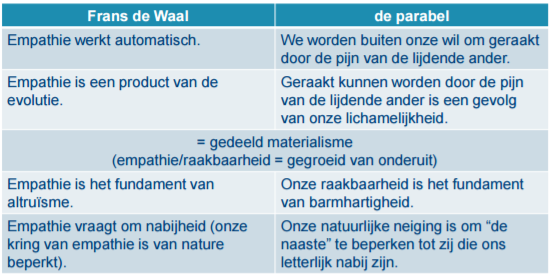
\includegraphics{figuur1.png} \\ 
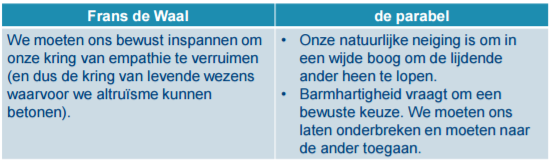
\includegraphics{figuur2.png}
\end{center}

\section{Stellingen}

\subsection{Wereldwijd hanteren de meeste wetenschappers het conflictmodel om de relatie tussen
religie en wetenschap te denken. }
\textcolor{red}{\textbf{Fout}}\\\\
Volgens de studie en de cijfers die we in de les hebben overlopen hanteren wereldwijd de meeste wetenschappers het kloofmodel om de relatie tussen religie en wetenschap te denken.
\subsection{Wereldwijd worden wetenschappers minder religieus door het beoefenen van hun
wetenschap.}
\textcolor{red}{\textbf{Fout}}\\\\
Volgens de studie en de cijfers die we in de les hebben overlopen voor de verschillende landen, claimde maximaal 22\% van de wetenschappers dat ze minder religieus werden door het beofenen van wetenschap, m.a.w. vond een grote meerderheid van de wetenschappers niet dat ze minder religieus werden door het beoefenen van wetenschap.

\subsection{Wetenschappers zijn altijd minder religieus dan de doorsneebevolking in hun land.}
\textcolor{red}{\textbf{Fout}}\\\\
Volgens de studie en de cijfers die we in de les hebben overlopen voor de verschillende landen, blijkt dat in sommige landen, zoals India en Taiwan, de wetenschappers geloviger zijn dan de doorsnee bevolking in hun land.

\subsection{Het conflictmodel staat het sterkst in contexten waarin het monotheïsme dominant is (of was).}

\subsection{Wereldwijd verdedigen de meeste wetenschappers een scheiding tussen religie en wetenschap.}
\textcolor{green}{\textbf{Juist}}\\\\
Volgens de studie en de cijfers die we in de les hebben overlopen hanteren wereldwijd de meeste wetenschappers het kloofmodel en zijn ze dus voor een scheiding tussen religie en wetenschap.

\subsection{Wetenschappers kunnen aanhanger zijn van het kloofmodel omdat ze er eigenlijk van uitgaan dat er een onoplosbaar conflict is tussen beide.}
\textcolor{red}{\textbf{Fout}}\\\\
Wanneer iemand ervanuit gaat dat er een onoplosbaar conflict is tussen beide, dan kan deze persoon geen aanhanger zijn van het kloofmodel, want het kloofmodel stelt juist dat wetenschap en religie twee totaal verschillende dingen kunnen zijn die niet met elkaar in verwarring kunnen worden gebracht.

\subsection{Francis Collins’ integratie van geloof en wetenschap vooronderstelt eigenlijk een voorafgaande scheiding tussen beide.}
\textcolor{green}{\textbf{Juist}}\\\\
Francis Collins verdedigt de theologische evolutie, dit betekend dat God de natuurwetten ingesteld heeft en dat de evolutie de manier is waarop hij zijn schepping realiseert. Aangezien hij stelt dat God zelf de wetten van de natuur heeft geschapen, is er geen onderscheid tussen wetenschap en geloof.

\subsection{Stephen Jay Gould verdedigt een scheiding tussen geloof en wetenschap maar eigenlijk is het NOMA-principe een verdoken vorm van conflictmodel.}
\textcolor{red}{\textbf{Fout}}\\\\
Integendeel, het NOMA-principe is de visie dat geloof en wetenschap twee verschillende domeinen zijn met eigen taak en autoriteit (wetenschap verklaart de werkelijkheid; geloof is bezig met levensvragen). Er kan daarom geen conflict zijn tussen beide.

\subsection{Wie vandaag een harmonie tussen geloof en natuurwetenschap nastreeft, bevordert volgens
Taede Smedes eigenlijk het conflict tussen beide.}
\textcolor{green}{\textbf{Juist}}\\\\
Om de integratie van geloof en wetenschap mogelijk te maken, moet de één op maat gesneden worden van de ander (of beide op maat van elkaar) (cf. het beeld van het procrustesbed). Hierdoor komen ze in elkaars vaarwater en ontstaan nieuwe conflicten.

\subsection{Het onderzoek van Sonja Lyubomirsky weerlegt de claim van Dirk De Wachter dat er weinig verband is tussen geluk en geld.}
\textcolor{red}{\textbf{Fout}}\\\\
Volgens Sonja Lyubomirsky wordt ons geluk vooral bepaald door onze genen en persoonlijkheid. Daarnaast spreekt ze ook over hedonistische adaptatie, het idee dat we een standaard geluksniveau hebben waarnaar we zeer snel terug zakken. Als we bijvoorbeeld een loonsvehooging krijgen dat zal ons dit een paar dagen, misschien zelfs een paar weken gelukkiger doen voelen, maar daarna zullen we terug vallen naar ons standaard geluksniveau.

\subsection{Het onderzoek van Sonja Lyubomirsky bevestigt de claim van Dirk De Wachter dat veel van ons geluk een kwestie is van geluk.}
\textcolor{green}{\textbf{Juist}}\\\\
Volgens Sonja Lyubomirsky is ons geluksniveau genetisch bepaald en kunnen we daarna nog weinig daaraan doen. Daarnaast is volgens haar ook de persoonlijkheid heel belangrijk, iemand die van nature de neiging heeft om alles negatiever te zien heeft het moeilijker om gelukkig te zijn. Daarnaast kan je je persoonlijkheid ook niet zomaar veranderen.

\subsection{Detraditionalisering betekent dat tradities verdwijnen.}
\textcolor{red}{\textbf{Fout}}\\\\
Detraditionalisering betekent dat traditionele opvattingen, gedragingen en omgangsvormen gerelativeerd worden. Ze verliezen hun dwingend karkater, maar verdwijnen niet. Ze veranderen van sociaal dwingende opties in mogelijke mogelijkheden.

\subsection{Individualisering betekent dat we met zijn allen egoïstischer worden.}
\textcolor{red}{\textbf{Fout}}\\\\
Individualisering betekent dat we meer zelf kunnen en moeten kiezen. Identiteitsconstructie een opdracht. We worden gedwongen de managers van ons leven te worden. Maar dit betekent niet automatisch dat we egoïstischer worden en enkel aan onszelf denken. 

\subsection{Individualisering betekent dat sociale ongelijkheid verdwijnt.}
\textcolor{red}{\textbf{Fout}}\\\\
Individualisering betekent dat we meer zelf kunnen en moeten kiezen. We moeten zelf kunnen kiezen tussen de mogelijkheden en kansen die we krijgen, maar dat betekend nog steeds niet dat iedereen dezelfde mogelijkheden en kansen krijgt. Sociale ongelijkheid is dus niet verdwenen maar binnen lagere bevolkingsklassen zijn er wel meer kansen dan vroeger.

\subsection{In de commandosamenleving zijn we volgens Byung-Chul Han allemaal onze eigen uitbuiter geworden.}
\textcolor{red}{\textbf{Fout}}\\\\
In een prestatie maatschappij zijn we allemaal onze eigen uitbuiter. In een prestatie maatschappij is er de prestatie druk, we zullen en moeten presteren. Dat zorgt ervoor dat we ons zelf gaan uitbuiten, onder deze druk worden we onze eigen uitbuiter. Zelfuitbuiting is nu eenmaal efficiënter dan uitbuiting door een ander omdat ze gepaard gaat met het gevoel van vrijheid.

\subsection{Byung-Chul Han verdedigt dat in de prestatiemaatschappij meer vrijheid en meer dwang hand in hand gaan.}
\textcolor{green}{\textbf{Juist}}\\\\
De vrijheid van autoriteiten leidt niet tot vrijheid, maar laat vrijheid en dwang samenvallen. Doordat we in een prestatie maatschappij onze prestaties willen maximaliseren verhogen we de druk op ons zelf. Dit resulteert uiteindelijk in zelfuitbuiting. Zelfuitbuiting is nu eenmaal efficiënter dan uitbuiting door een ander omdat ze gepaard gaat met het gevoel van vrijheid.

\subsection{Volgens Paul Verhaeghe heeft onze identiteit een biologisch-evolutionair fundament.}
\textcolor{green}{\textbf{Juist}}\\\\
Paul Verhaeghe benadrukt dat onze identiteit een constructie is vanuit de omgeving. Maar bouwen doe je steeds op een fundament en dat fundament is biologisch-evolutionair: de mens als een sociaal en hiërarchisch wezen dat in staat is tot samenwerking en competitie. 

\subsection{Volgens Paul Verhaeghe is onze identiteit een sociale constructie en heeft die bijgevolg geen biologisch-evolutionair fundament.}
\textcolor{red}{\textbf{Fout}}\\\\
Paul Verhaeghe benadrukt dat onze identiteit een constructie is vanuit de omgeving. Maar bouwen doe je steeds op een fundament en dat fundament is biologisch-evolutionair: de mens als een sociaal en hiërarchisch wezen dat in staat is tot samenwerking en competitie. 

\subsection{Volgens Paul Verhaeghe bewijst adoptie dat onze identiteit geen biologisch-evolutionair fundament heeft.}
\textcolor{red}{\textbf{Fout}}\\\\
Adoptie bewijst dat onze identiteit niet enkel een biologisch-evolutionair fundament heeft. Onze identiteit wordt namelijk ook mee geconstrueerd door onze omgeving. Maar bouwen doe je steeds op een fundament en dat fundament is biologisch-evolutionair: de mens als een sociaal en hiërarchisch wezen dat in staat is tot samenwerking en competitie.

\subsection{Hoe we denken over onszelf (m.a.w. ons zelfbeeld) is volgens Paul Verhaeghe een constructie vanuit de omgeving.}
\textcolor{green}{\textbf{Juist}}\\\\
De verhouding die ik aanneem tegenover mezelf is bepaald door wat ik van anderen gehoord heb over mezelf tijdens de periode waarin mijn identiteit gevormd werd. Cf. reactie van moeder op actieve baby in haar buik: “het is nu al een lastige ADHD’er” vs. “er zit pit in, mooi zo”.
\subsection{Empathie vraagt om sterk ontwikkelde cognitieve vermogens en komt bijgevolg slechts bij weinig dieren voor.}
\textcolor{red}{\textbf{Fout}}\\\\
De meest basale vorm van empathie is emotionele aanstekelijkheid, het overnemen van de gemoedstoestand van een ander individu. Bvb. één vogel schrikt en ze vliegen allemaal weg. Dit kan zonder begrip van de situatie van de ander en dus zonder sterke cognitieve vermogens. 

\subsection{Gerichte hulp is wijdverbreid in het dierenrijk en moet bijgevolg reeds vroeg in de evolutie van het leven ontstaan zijn.}
\textcolor{red}{\textbf{Fout}}\\\\
Gerichte hulp betekent dat we in staat zijn in te schatten wat er met een ander aan de hand is en wat hij/zij nodig heeft. Dit vraagt om toegenomen intelligentie en komt daarom slechts bij enkele diersoorten voor (bijvoorbeeld mensapen, olifanten en dolfijnen). 

\subsection{Volgens de cursus is een gezonde dosis egocentrisme noodzakelijk.}
\textcolor{green}{\textbf{Juist}}\\\\
De mens is een kwetsbaar en sterfelijk wezen dat de taak heeft zich in het bestaan te handhaven. We moeten moeite doen om in leven te blijven, dat gaat niet zomaar. We moeten dus bekommerd zijn om onszelf, met onszelf inzitten en dus aan onszelf denken (= zelfzorg). 

\subsection{Het feit dat de priester en de leviet in de parabel van de Barmhartige Samaritaan met een wijde boog om de gewonde man heen lopen maakt duidelijk dat ze hem niet hebben zien liggen.}
\textcolor{red}{\textbf{Fout}}\\\\
De priester en de leviet lopen juist met een boog om de gewonde man omdat ze hem hebben zien liggen (anders zouden ze rechtdoor gelopen zijn). Ze worden door hem geraakt en weten zich geappelleerd, maar kiezen ervoor deze verstoring van hun zijnspoging te negeren.

\subsection{De verschijning van de lijdende ander leidt tot het einde van mijn vrijheid.}
\textcolor{red}{\textbf{Fout}}\\\\
De noodlijdende ander onderbreekt mijn zelfzorg. Als kwetsbaar en lichamelijk wezen word ik door zijn kwetsbaar en gekwetst lichaam geraakt. Ik verlies mijn
vrijheid van initiatief, maar behoud wel mijn vrijheid van antwoord. 

\subsection{Naastenliefde betekent dat je iedereen even sympathiek moet vinden.}
\textcolor{red}{\textbf{Fout}}\\\\
Naastenliefde betekent barmhartigheid tonen, ook als de noodlijdende ander niet tot onze kring van empathie hoort en ons eerder afstoot dan aantrekt. Dus ongeacht of we sympathie voor deze persoon hebben of niet.

\subsection{Volgens de cursus is het absurd om van de naastenliefde een gebod te maken.}
\textcolor{red}{\textbf{Fout}}\\\\
Naastenliefde is geen erotisch verlangen of vriendschap. Het betekent barmhartigheid tonen, ook als de noodlijdende ander niet tot onze kring van empathie hoort en ons eerder afstoot dan aantrekt. Dit doen we niet van nature en daarom is de naastenliefde een gebod.

\subsection{De naastenliefde is een gebod omdat ze tegennatuurlijk is.}
\textcolor{green}{\textbf{Juist}}\\\\
Naastenliefde is geen erotisch verlangen of vriendschap. Het betekent barmhartigheid tonen, ook als de noodlijdende ander niet tot onze kring van empathie hoort en ons eerder afstoot dan aantrekt. Dit doen we niet van nature en daarom is de naastenliefde een gebod.

\subsection{De parabel van de Barmhartige Samaritaan leert ons alles over de ethische verhouding tussen mensen.}
\textcolor{red}{\textbf{Fout}}\\\\
De parabel van de Barmhartige Samaritaan leert ons veel over barmhartigheid en hoe we de noodlijdende ander moeten helpen. Toch zegt de parabel bijna niets over de grenzen van de barmhartigheid.

\subsection{De parabel van de Barmhartige Samaritaan presenteert de Samaritaan waar de parabel naar genoemd is als een model van totale barmhartigheid.}
\textcolor{red}{\textbf{Fout}}\\\\
De Samaritaan begrenst zijn barmhartigheid. Hij roept de hulp in van een ander (de herbergier, tegen betaling). Zijn primaire verantwoordelijkheid verdwijnt ook niet. Na de nodige voorzieningen getroffen te hebben, zet hij zijn reis verder (hij geeft zijn plannen niet op).

\section{Korte open vragen}

\subsection{Waarom zijn we de colleges begonnen met de reflectie van Carl Sagan over Pale Blue Dot?}
De colleges zijn begonnen met de reflectie van Carl Sagan over Pale Blue Dot, omdat de afbeelding aantoont dat wij maar een zeer klein puntje zijn in een gigantisch heelal waar heel veel niet over geweten is.\\ Dit doet bij Sagan ook een hele boel vragen reizen "Waarom zou een God in ons geïnteresseerd zijn?", "Wat is nu de zin van het leven?", "Hoe komt het heelal er?", "Wat is de rol van wetenschap?", "Maak wetenschap ons gelukkiger?".\\ De video was dus een perfecte keuze om de lessen te starten omdat ze ons doet stilstaan en ons nieuwsgierig maakt naar de essentiele vragen van deze cursus.

\subsection{In 1986 publiceerde Richard Dawkins een boek met als titel De blinde horlogemaker. Wat is de betekenis van deze titel?}
De titel van het boek verwijst naar natuurlijke selectie.  William Paley schreef in zijn boek Natural Theology, dat het bestaan van een complex wezen zoals de mens het bestaan van een schepper bevestigt, net zoals het bestaan van een complex horloge het bestaan van een horlogemaker bevestigt. Dawkins haalt in zijn boek de theorie van Paley onderuit, omdat de mens complex is geworden door natuurlijke selectie, door de willekeurige mutaties en de cumulatieve selectie daarop. De natuur is dus eigenlijk een blinde horlogemaker die zonder enig inzicht of planning een horloge schept.

\subsection{Wat is de parabel van de onzichtbare tuinman en hoe functioneerde zij binnen de cursus?}
De parabel van de onzichtbare tuinman gaat over twee mannen die na lange tijd terug keren naar hun huis en opmerken dat hun tuin er nog steeds onderhouden uitziet. Eén van de twee mannen is er dan ook van overtuigd dat er een tuinman is die hun tuin onderhoudt als ze er niet zijn, tewijl de andere man denkt dat dit niet het geval is. Om te weten wie nu gelijk heeft doen ze een hoop testen, maar niets biedt uitsluitsel. De ene man heeft argumenten waarom de tuinman wel bestaat en de andere heeft argumenten waarom de tuinman niet bestaat. Het is een onoplosbare discussie, want beide mannen kijken met een andere bril. \\
In de cursus komt dit verhaal terug om aan te tonen dat het moeilijk is om over geloof te discusiëren en dat je het bestaan van God niet kan bewijzen, net zoals het bestaan van de tuinman niet kan worden bewezen. En dat het daarom moeilijk is om over het bestaan van God te discusiëren.

\subsection{Waarom hebben we het tijdens de colleges over de sluipwespen gehad?}
Sluipwespen zijn wespen die rupsen een gif toedienen en er vervolgens hun eitjes in de rups leggen. Het gif zorgt ervoor dat de rups gebrainwashed is en de eitjes van de wesp verdedigt, de rups zal ook sterven nadat de larven uit de eitjes zijn gekropen. \\ 
Het is dus vrij gruwelijk gedrag van de natuur, juist daarom claimed Gould dat we de natuur niet als basis mogen nemen voor onze moraal. De natuur is soms gruwelijk en daarom hebben we geloof nodig. Dit is één van de redenen waarom Gould pleit voor een scheiding tussen geloof en wetenschap.
\subsection{Wat wordt bedoeld met “resonanties” tussen geloof en wetenschap? }
 “Resonantie” is een term uit de muziekwereld (eigenlijk uit de natuurkunde) en betekent zoveel als
“meetrillen” of “samen klinken”. Hier wordt de term gebruikt om aan te
geven dat er tussen geloof en wetenschap op een bepaald punt een
zekere verwantschap gevoeld kan worden, maar ook niet meer dan dat

\subsection{Hoe functioneerde het fragment uit Tarkovski’s Nostalghia in de opbouw van de colleges en wat hebben we er uit geleerd?}
Het fragment gaat over Eugenia die niet kan knielen, maar wel wil. Ze zou wel willen geloven, maar ze kan het niet. De vraag is of ze gokt op het bestaan van God (en tijdens haar leven even een effort doet) en eeuwig geluk na het leven heeft of dat ze ervan uitgaat dat God niet bestaat en later eeuwig ongelukkig is als hij toch zou bestaan. Ze is dus eigenlijk opzoek naar geluk. Dit fragement maakt de overgang naar het volgende onderwerp in de cursus, namelijk geluk. Wereldwijd vinden mensen geluk belangrijk, maar de vraag is of geluk wel het belangrijkste is. Nog bijkomende vragen zijn dan of wetenschap ons gelukkig kan maken en of het eigenlijk wel goed is om gelukkiger te willen worden.

\subsection{Dirk De Wachter pleit voor een beetje ongelukkig zijn. Waarom doet hij dat? Wat is er mis met gelukkig willen zijn? Welke paradox stelt De Wachter vast met betrekking tot de manier waarop mensen omgaan met geluk en ongeluk? }
Volgens Dirk De Wachter is gelukkig zijn in onze maatschappij een obsessie geworden. We hebben van extreem gelukkig zijn het doel van het leven gemaakt. Het is niet meer normaal hoe gelukkig we willen zijn. Dat is een vergissing. Extreem geluk najagen is de koninklijke weg naar een depressie. Het doel van het leven is niet gelukkig zijn, maar een goed leven leiden, dan komt geluk daar wel bij. Omdat we zo gelukkig willen zijn, kunnen we niet meer om met ongeluk. Geluk is
maakbaar en te koop. Het is onze verdienste, we hebben er voor gewerkt, het komt ons toe, we hebben er recht op. Ongeluk past niet in dat plaatje en daarom maken we er ziekte van. Dan zijn we plots ons brein en vragen we aan de psychiater om ons beter te maken met pillen zodat we ons opnieuw gelukkig kunnen voelen. De Wachter wijst er verder ook nog op dat geluk veel te maken heeft met geluk, met “platte chance”.

\subsection{Wat zijn de belangrijkste inzichten van Sonja Lyubomirsky over geluk?}
Volgens Sonja Lyubomirsky is geluk grotendeels genetisch bepaald. We hebben een bepaald geluksniveau waarmee we geboren worden. Daarnaast speelt volgens haar ook onze persoonlijkheid een grote rol. Mensen die van nature de neiging hebben om alles iets negatiever te zien zullen het ook moeilijker hebben om gelukkig te zijn. Daarnaast spreekt ze ook over hedonistische adaptatie het feit, dat we beschikken over een standaard geluksniveau, dat door onze genen wordt bepaald, waarnaar we steeds zullen terugvallen. Volgens haar zorgt een loonsverhoging, dus maar voor een tijdelijke verhoging van geluk en zullen we na een bepaalde tijd steeds terug vallen naar dat standaard geluksniveau. Tot slot spreekt Sonja ook nog over de twaalf geluksactiviteiten, dit gaat over het feit dat we een goed mens moeten zijn en niet zozeer geluk moeten nastreven. Als we een goed mens zijn dan volgt het geluk vanzelf.

\subsection{Wat is individualisering en wat het is het verband tussen individualisering en prestatiedwang?}
Individualisering betekent dat we meer zelf kunnen en moeten kiezen. We moeten zelf de managers van ons leven worden. Individualisering houdt vrijmaking in. Er liggen voor elk individu vele mogelijkheden open. We kunnen zelf kiezen welke we willen benutten. Er zijn dus meer mogelijkheden om te kiezen voor andere invullingen van onze identiteit, gebaseerd op alternatieve verhalen (= separatie).  \\
Individualisering zorgt voor het onbegrenst kunnen van het individu. We komen hierdoor terecht in een prestatiemaatschappij waarin we de opdracht hebben om te presteren in de laatmoderne samenleving van de hardwerkende burger. De vrijheid van autoriteiten leidt niet tot vrijheid, maar laat vrijheid en dwang samenvallen.  We willen onze prestaties maximaliseren en verhogen de druk op ons zelf. Dit resulteert uiteindelijk in zelfuitbuiting. Zelfuitbuiting is nu eenmaal efficiënter dan uitbuiting door een ander omdat ze gepaard gaat met het gevoel van vrijheid.

\subsection{Waarom werd in de cursus verwezen naar de inzichten van Jan Blommaert?}
Jan Blommaert heeft een boekje geschreven met als titel, Let op je woorden. Daarin wijst hij erop dat taalgebruik nooit neutraal is, maar dat het altijd de bedoeling heeft om de werkelijkheid voor te stellen op een manier die de spreker goed uitkomt. Het is dus belangrijk om altijd te vragen: Wiens woorden zijn dit eigenlijk? Welke belangen zitten er achter? Wie wordt er beter van als we dit woord zonder nadenken gebruiken? Zo is er het woord “loonlast”, dat suggereert dat lonen een last zijn en dus best zo laag mogelijk gehouden worden. Maar voor wie is een hoger loon een last? Toch niet voor wie dat loon ontvangt? Het
woord “loonlast” drukt dus duidelijk een bepaald belang uit, namelijk het belang van zij die de lonen betalen en die er dus baat bij hebben dat iedereen, ook zij die de lonen ontvangen, denkt in hun termen van lonen als een last. Dit sluit aan bij de visie van Paul Verhaeghe die stelt dat taal ons denken, onze werkelijkheid en onze identiteit bepaalt. 

\subsection{Wat is de visie van Paul Verhaeghe op identiteit?}
Volgens Paul Verhaeghe is onze identiteit een constructie vanuit de omgeving. Hij bewijst dit door te zeggen dat de identiteit en het karakter van adoptie kindern gelijkt op dat van de adoptie ouders. Het adoptie kind zijn identiteit is dus deels bepaald door de adoptie ouders ookal hebben ze geen biologische connectie. Toch wordt die identiteit volgens hem steeds opgebouwd vanuit een fundament en dat fundament is biologisch-evolutionair: de mens als een sociaal en hiërarchisch wezen dat in staat is tot samenwerking en competitie. 

\subsection{Wat kenmerkt volgens Paul Verhaeghe het neoliberalisme? Wat doet het neoliberalisme met het egoïsme? Welk moreel onderscheid maakt het neoliberalisme?}
Het neoliberalisme wordt volgens Verhaeghe gekenmerkt door een nieuwe dwingende morele norm, met name die van de efficiëntie of meer winst op korte termijn door het installeren van meer concurrentie tussen de mensen (cf. het ‘Rank and Yank’-systeem). Het neoliberalisme herdefinieert he egoïsme in drie stappen: (1) egoïsme is natuurlijk, (2) egoïsme is rationeel en de beste strategie, en (3) egoïsme is zelfs de hoogste deugd want als we met z’n allen egoïstisch zijn zal het uiteindelijk in het voordeel zijn van iedereen. Het ideaal van het neoliberalisme is de entrepreneur, het hardwerkwerkende, flexibele,
efficiënte individu dat uit is op winst en daarom rationeel en instrumenteel-egoïstisch. Daar tegenover staat de profiteur, de loser die niet bijdraagt aan de maatschappij en bovendien nog profiteert van wat de hardwerkende entrepreneurs opgebouwd hebben.

\subsection{Jan Rosier omschrijft de huidige generatie als “een generatie controlefreaks”. Wat bedoelt hij hier mee en op welke manier bevestigt zijn analyse de visie van Paul Verhaeghe op het neoliberalisme?}
Rosier stelt vast dat onze cultuur doordrenkt is geraakt van het “managementdenken”, de idee dat alles onder controle te brengen en te houden is. We denken dat succes uitsluitend een kwestie is van wat we als individu doen en beslissen. Er is geen ruimte meer voor pech, het onverwachte, het noodlot. Dit sluit aan bij de visie van Verhaeghe die stelt dat het neoliberalisme een dwingende invulling heeft gegeven aan maakbaarheid en verantwoordelijk. Alles is vandaag slechts een kwestie van inspanning. Je kan én moet het maken. Als je mislukt, dan is het je eigen schuld, want je hebt niet hard genoeg je best gedaan (dit
is het zogenaamde “individuele schuldmodel”). Daarom plannen we ons te pletter. Want we willen geen mislukkeling, geen profiteur zijn. De overtuiging dat alles slechts een kwestie van inspanning is, zorgt er ook voor dat we geen tijd meer hebben voor solidariteit met degenen voor wie het minder gaat. Ze moeten maar beter hun best doen.

\subsection{Waarom sluit de bespreking van Frans de Waal aan op de bespreking van het neoliberalisme?}
Frans de Waal zegt dat er twee niveaus bestaan. Het niveau van de natuurlijke selectie, de concurrentie, competitie, de strijd om het bestaan, dit is het fundamentele niveau. Het tweede niveau is het niveau van de onmiddellijke motivatie van ons gedrag. Niet omdat het mechanische van de natuurlijke selectie aanwezig is, dat we ons daarom in ons gedrag moeten laten lijden door dat fundamentele niveau, dit gebeurd daarentegen wel in het neoliberalisme. Hij geeft dus een reden waarom we ons niet zouden moeten toeleggen op dat neoliberalisme.

\subsection{Leg uit: “Empathie is gelaagd als een Russisch poppetje” (Frans de Waal).}
Voor Frans de Waal is empathie te vergelijken met een Russisch poppetje met drie lagen. De binnenste laag is de oudste, de andere lagen zijn er dan later rond gekomen. Binnenste laag is de emotionele aanstekelijkheid. Deze is wijdverspreid in het dierenrijk, bv. muizen die pijn voelen als ze een andere muis pijn zien lijden. Tweede laag is er daarna bijgekomen, het geven van troost. Iemand die niet betrokken is in een gevecht gaat proberen iemand die betrokken is in het gevecht zijn gemoedstoestand te verbeteren. Derde laag, deze is het minst wijd verspreidt, de empatische perspectiefname. Dit is het instaat zijn om in te schatten wat een ander nodig heeft. Bijvoorbeeld een duiker die in de problemen is en wordt gered door een dolfijn. De drie lagen van empathie vormen voor Frans de Waal de bron van altruïsme. Altruïsme is het doen van iets dat geen voordeel of zelfs een nadeel oplevert in de strijd om het bestaan. 

\subsection{Wat is altruïsme en op welke manier is empathie hiervan het evolutionair fundament?}
Altruïsme betekent iets doen dat geen voordeel of zelfs een nadeel oplevert in de strijd om het bestaan. Dit vraagt om een sterke en onmiddellijke drijfveer. Volgens Frans De Waal biedt empathie deze drijfveer. Empathie betekent de nood/pijn van een ander voelen. Empathie gebeurt automatisch en levert als zodanig een voordeel op in de strijd om het bestaan (een empathische moeder die de nood van haar kroost voelt, zal een betere moeder zijn). Dankzij het vermogen de pijn van een ander te voelen en, bij toegenomen cognitieve vermogens, te weten wat hij nodig heeft, kunnen we komen tot altruïstische daden: bvb. chimpansee springt in het water om soortgenoot van verdrinking te redden, ook al doet hij dit op gevaar voor eigen leven want chimpansees kunnen niet zwemmen en is dit eigenlijk niet rationeel (twee verdronken chimpansees is erger dan één verdronken individu).

\subsection{Leg uit: “Het is niet omdat biologen het voortdurend over concurrentie hebben dat ze concurrentie aanbevelen” (Frans de Waal). }
Het is belangrijk om een onderscheid te maken tussen twee niveaus. Het niveau van de natuurlijke selectie, de concurrentie, competitie, de strijd om het bestaan, dit is het fundamentele niveau. Het tweede niveau is het niveau van de onmiddellijke motivatie van ons gedrag. Niet omdat het mechanische van de natuurlijke selectie aanwezig is, dat we ons daarom in ons gedrag moeten laten lijden door dat fundamentele niveau.

\subsection{De aanleiding voor het vertellen van de parabel van de Barmhartige Samaritaan is de vraag van een wetgeleerde. Om welke vraag gaat het hier? Waarom is dat een strikvraag? Hoe ontsnapt Jezus aan de valstrik?}
De wetgeleerde vraagt aan Jezus wat hij moet doen om eeuwig te leven. Jezus antwoord hem dan dat hij zijn naasten moet liefhebben zoals zichzelf, dat hij moet houden van God en zijn naasten. De geleerde vraagt vervolgens wie zijn naasten zijn, zijn dat dan de meest nabije? Maar wanneer je naasten alleen degenen zijn die het meest nabij zijn, dan riskeer je om mensen uit te sluiten. Wanneer je naasten enkel je vrienden zijn, dan sluit je de mensen uit die het het meest nodig hebben, de bedelaar in het station bijvoorbeeld. Jezus heeft door dat hij hem in de val probeerd te lokken. Jezus lost dit op door de parabel van de barmhartige samaritaan te vertellen en te zeggen dat je naaste moet worden van iedereen die dat nodig heeft.

\subsection{Waarom is de naastenliefde een gebod?}
Naasteliefde is geen gevoel, niet zoals verliefd zijn, niet iets dat je voelt. Het is ook geen erotisch verlangen, je kan in de andere geen wederhelft vinden, het is geen leegte die door een ander kan worden opgevuld. Het is ook geen vriendschap, vriendschap heeft te maken met wederkerigheid, er is een evenwicht tussen geven en nemen. Bij vriendschap is er ook vrijwilligheid, je kiest zelf met wie je vrienden bent en dat heeft vaak te maken met zelfde intresses. Bij naasteliefde is dat niet, je kiest het niet, het is bijna tegennatuurlijk. Daarom dat het wel een gebod moet zijn.

\subsection{In de hedendaagse bewerking van de parabel van de Barmhartige Samaritaan die tijdens de les getoond werd, wordt ons aangeraden iedereen lief te hebben alsof ze dood zullen zijn tegen middernacht. Hoe kunnen we dit begrijpen?}
We hebben deze raad geduid als een hedendaagse variant van de opvatting van de joodse rabbijnen dat ware barmhartigheid erin bestaat iemand lief te hebben alsof hij dood is. Een dode kan niets meer terugdoen. Alles wat we voor hem/haar doen is volstrekt gratuit, asymmetrisch, niet-wederkerig. Wat we doen, doen we niet met het oog op er later iets voor terugkrijgen (er is geen “return upon investment” mogelijk, geen geven om te krijgen). De raad in het filmfragment wijst ook op het feit dat er van ons onmiddellijke actie verwacht wordt. We kunnen het betonen van barmhartigheid niet uitstellen, want morgen zal die persoon er niet
meer zijn en zullen we hem in zijn sterven alleen gelaten hebben, terwijl barmhartigheid er juist in bestaat de noodlijdende ander in zijn/haar sterven niet alleen te laten. 

\subsection{Bespreek de grenzen van de barmhartigheid in verwijzing naar Genesis, hoofdstuk 12.}
Het verhaal van Abraham \& Sarah in Egypte. Rabijnen die over dit verhaal nadachten vonden twee grenzen aan barmhartigheid.
\begin{enumerate}
\item De eigen persoonswaarde en integriteit als grens. Niemand mag zichzelf als middel gebruiken om een doel te bereiken. Ookal is het doel om iemand anders te redden. Je mag er niet mee instemmen jezelf louter als middel te behandelen en zo jezelf te vernietigen. Je kan dit ook terug vinden in het scheppingsverhaal, iedereen is geschapen door god en iedere mens  bezit een onvervreemdbare waardigheid, iedere mens is beeld van god en niemand kan gedwongen worden en niemand kan en mag dat beeld van god in zichzelf gaan vernietigen, ook niet als het is om een ander te redden.\\ Sarah had door zich over te leveren aan de pharao, haar lichamelijke integriteit op het spel gezet, het beeld van god in zichzelf vernietigd en ging daarbij over de eerste grens.
\item De verantwoordelijkheid in de derde persoon, de verantwoordelijkheid voor de derden. De derden kunnen zowel mensen zijn die gescheiden van ons zijn in de ruimte, als gescheiden in de tijd. De tragiek van de goedheid, door goed te doen voor één persoon, je te focussen op exact één persoon, loop je de kans de andere, derden die jouw zorg en aandacht ook nodig hebben vergeet en dat je ook de gevolgen voor die derden vergeet. De barmhartigheid moet dus begrensd worden door de rechtvaardigheid.\\ De derden in het verhaal van Sarah en Abraham zijn volgens de rabijnen, het uitverkorene volk dat er nog niet is. Sarah heeft door vrouw te worden van de pharao de toekomstige generaties in het gedrang gebracht.
\end{enumerate}
\end{document}